\documentclass[conference]{IEEEtran}

%!TEX root = main.tex
\usepackage[utf8]{inputenc}
\usepackage[T1]{fontenc}

\usepackage{listings}
\lstset{
  basicstyle=\ttfamily\scriptsize,
  breaklines
}

% Notes
\usepackage{manfnt}
\def\hang{\hangindent19pt}
\def\d@anger{\medbreak\begingroup\clubpenalty=10000
 \def\par{\endgraf\endgroup\medbreak} \noindent\hang\hangafter=-2
 \hbox to0pt{\hskip-\hangindent\dbend\hfill}\small}
\outer\def\danger{\d@anger}

% inline references
\usepackage{prettyref}
\newrefformat{cha} {Chapter~\ref{#1}}
\newrefformat{sec} {Section~\ref{#1}}
\newrefformat{fig} {Fig.~\ref{#1}}
\newrefformat{tab} {Table~\ref{#1}} 
\newrefformat{lst} {Listing~\ref{#1}} 
\newrefformat{eq}  {Eq.~\ref{#1}}
\newrefformat{ex}  {Example~\ref{#1}}

%%% Local Variables:
%%% mode: latex
%%% TeX-master: "main"
%%% End:

%!TEX root = main.tex
\usepackage{tikz}
\usetikzlibrary{backgrounds,positioning,fit}

% overview of the architecture
\newcommand{\tikzarchitecture}{
  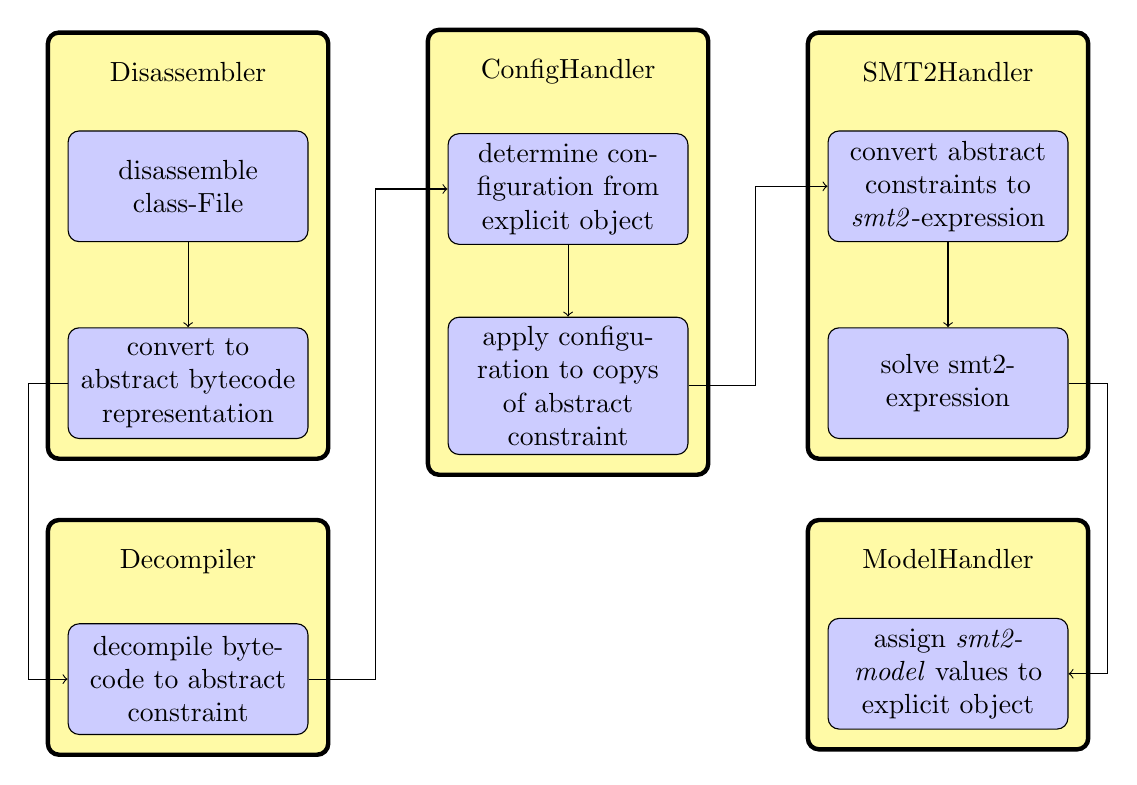
\begin{tikzpicture}[node distance=2.5cm]
    \tikzstyle{block} = [rectangle, draw, fill=blue!20, text width=8em,
        text centered, rounded corners, minimum height=4em]
    \tikzstyle{line} = [draw, ->]
    \tikzstyle{container} = [rectangle, draw, ultra thick, rounded corners,
        inner sep=.25cm, fill=yellow!35]
    \tikzstyle{containertitle} = [minimum width=8em]

    % Disassembler
    \node[minimum width=8em] (disname) {Disassembler};
    \node[block, below=.5cm of disname] (disassemble) {disassemble class-File};
    \node[block, below of=disassemble] (convert) {convert to abstract bytecode
        representation};
    \draw[line] (disassemble) -- (convert);
    \begin{scope}[on background layer]
      \node[container,fit=(disname) (disassemble) (convert)] (disassembler) {};
    \end{scope}
    % Decompiler
    \node[containertitle,below=1cm of disassembler] (decname) {Decompiler};
    \node[block, below=.5cm of decname] (decompile) {decompile bytecode to
        abstract constraint};
    \begin{scope}[on background layer]
      \node[container,fit=(decname) (decompile)] (disassembler) {};
    \end{scope}
    % AssignmentHandler
    \node[containertitle,right=2cm of disname] (confname) {ConfigHandler};
    \node[block, below=.5cm of confname] (config) {determine configuration from
        explicit object};
    \node[block, below of=config] (apply) {apply configuration to copys of
        abstract constraint};
    \draw[line] (config) -- (apply);
    \begin{scope}[on background layer]
      \node[container,fit=(confname) (config) (apply)] (confighandler) {};
    \end{scope}
    % AssignmentHandler
    \node[containertitle,right=2cm of confname] (smt2name) {SMT2Handler};
    \node[block, below=.5cm of smt2name] (smt2converter) {convert abstract
        constraints to \emph{smt2}-expression};
    \node[block, below of=smt2converter] (smt2solver) {solve smt2-expression};
    \draw[line] (smt2converter) -- (smt2solver);
    \begin{scope}[on background layer]
      \node[container,fit=(smt2name) (smt2converter) (smt2solver)]
          (smt2handler) {};
    \end{scope}
    % Allocator
    \node[containertitle,below=1cm of smt2handler] (modname) {ModelHandler};
    \node[block, below=.5cm of modname] (assigner) {assign \emph{smt2-model}
        values to explicit object};
    \begin{scope}[on background layer]
      \node[container,fit=(modname) (assigner)]
          (modelhandler) {};
    \end{scope}

    \draw[line] (convert.west) -| ++(-.5,0) |-  (decompile.west);
    \draw[line] (decompile.east) -- ++(.85,0) |- (config.west);
    \draw[line] (apply.east) -- ++(.85,0) |-  (smt2converter.west);
    \draw[line] (smt2solver.east) -| ++(.5,0) |-  (assigner.east);
  \end{tikzpicture}
}

\newcommand{\tikzjvm}{
  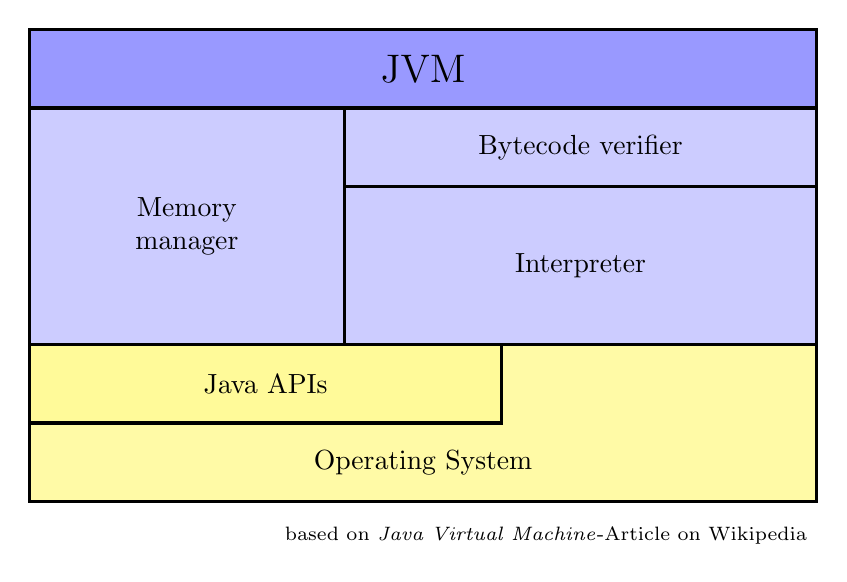
\begin{tikzpicture}
    \draw[very thick,fill=yellow!35] (0,0) rectangle (10,6);

    \draw[very thick] (0,2) rectangle (10,5);
    \draw[very thick,fill=blue!40] (0,5) rectangle (10,6) node[midway,
      align=center] {\Large JVM};
    \draw[very thick,fill=blue!20] (0,2) rectangle (4,5) node[midway,
      align=center] {Memory\\manager};
    \draw[very thick] (4,2) rectangle (10,5);
    \draw[very thick,fill=blue!20] (4,4) rectangle (10,5) node[midway,
      align=center] {Bytecode verifier};
    \draw[very thick,fill=blue!20] (4,2) rectangle (10,4) node[midway,
      align=center] {Interpreter};
    \draw[very thick,fill=yellow!40] (0,1) rectangle (6,2) node[midway,
      align=center] {Java
      APIs};
    \draw[very thick] (0,0) rectangle (10,2);
    \draw[draw=none] (0,0) rectangle (10,1) node[midway,align=center]
      {Operating System};

    \draw[draw=none] (0,0) rectangle (10,-.2) node[anchor=north east]
      {\scriptsize based on \emph{Java Virtual Machine}-Article on Wikipedia};
  \end{tikzpicture}
}

%%% Local Variables:
%%% mode: latex
%%% TeX-master: "main"
%%% End:


\title{Formal Methods For Everyone}
\author{%
  \IEEEauthorblockN{Author 1 \quad Author 2 \quad Author 3}
  \IEEEauthorblockA{%
    $^1$ Department of Mathematics and Computer Science, University of Bremen,
    Germany \\
    $^2$ Cyber-Physical Systems, DFKI GmbH, Bremen, Germany
  }
}

\begin{document}

\maketitle

\begin{abstract}
\end{abstract}

\section{Introduction}
\label{sec:introduction}

\danger Mathias

\section{Related Work}
\label{sec:related-work}

\danger Mathias, Sketching, Software synthesis, Model finding, \dots

\section{Preliminaries}
\label{sec:preliminaries}

\ldots

\subsection{Java Virtual Machine}
\label{sec:prelim_jvm}

The \emph{Java Virtual Machine~(JVM)} is the interpreter for compiled java
code. The JVM is the part of the \emph{Java Runtime Environment~(JRE)}, that
abstracts from the respective platform, so the interpreted programs are
platform-independent.

As shown in \prettyref{fig:jvm} the JVM consist of three important parts: The
\emph{memory manager} manages all accesses to the memory of the running
program. Before interpreting the bytecode of the given program, it is checked
for syntactic faults by the \emph{bytecode verifier}. Afterwards the bytecode
is interpreted by the \emph{Interpreter} component. Together the JVM and the Java~APIs represent the JRE.

\begin{figure}[!ht]
  \centering
  \resizebox{.8\columnwidth}{!}{\tikzjvm}
  \caption{Java Virtual Machine}
  \label{fig:jvm}
\end{figure}

The interpreted binary code is called \emph{java bytecode}. This bytecode is
similar to the Assembler-Code on regular processors or microcontrollers.

For example for a method thats adds two to an integer, given as parameter to
the method, the java bytecode looks like the one given in
\prettyref{lst:example_bytecode_add_up_2}.

\begin{bytecodelst}[caption=Java bytecode list for a Method that adds up 2,
    label=lst:example_bytecode_add_up_2]
public int add2(int);
  Code:
   0: iload_1
   1: iconst_2
   2: iadd
   3: ireturn
\end{bytecodelst}

In line three (\texttt{iload\_1}) the first integer parameter of the method is
pushed on top of the methods stack. In the next line the integer
constant~\texttt{2} is pushed on top of the stack. And in line five the two top
integer elements are pulled down and their sum is re-pushed on top of the
methods stack again. Finally the top integer element of the stack is returned.

A description for all bytecode instructions, in this case for Java~7, is shown
in~\cite{LindholmYBB11}.

\subsection{Java Class File Disassembler}
\label{sec:prelim_javap}

The \emph{Java Class File Disassembler~(javap)} is a class file disassembler,
that reconstructs the bytecode from one or more java class files. Based on the
options set with the command call, the tool prints the disassembled class out
to \texttt{stdout}. One of the options is \texttt{-c}, to get the disassembled
code of the methods, besides their signatures. To disassemble additionally all
private methods, the option \texttt{-p} is used.

The program is delivered with the \emph{Java Development Kit~(JDK)}. Since
JDK~1.7 it also reconstructs the generic values of methods, fields and classes
of class-files that have been compiled with a compiler of JDK~1.7 or higher.

\subsection{Satisfiability Modulo Theories}
\label{sec:prelim_smt}

\danger Mathias

\section{Example -- Vertex Coloring}
\label{sec:example_vertex_coloring}

A \emph{vertex coloring} is an assignment of colors to each vertex of a graph
with the restriction that two adjacent vertices must not have the same color.
A graph that can be assigned with a vertex coloring with \emph{k} colors is
\emph{k-colorable}.

\begin{javalst}[label=lst:graph_coloring,caption=Graph-coloring example]
public class Vertex {
  private int color;
  ...
}

public class Edge {
  private Vertex vertex1;
  private Vertex vertex2;
  ...
}

public class Graph {
  private Collection<Vertex> vertices;
  private Collection<Edge> edges;

  public boolean adjacentsColorsDiffer() {
    for (Edge e : this.edges)
      if (e.getVertex1().getColor() == e.getVertex2().getColor())
        return false;
    return true;
  }
  ...
}
\end{javalst}

In the example java implementation in \prettyref{lst:graph_coloring} there are
the two data classes \texttt{Vertex} and \texttt{Edge} that are collected to a
graph within the \texttt{Graph} class. The graph class also contains the
method for checking for a valid assignment of the \emph{color} variable of the
vertices (\texttt{adjacentsColorsDiffer}).

For getting a coloring for a given graph, there are basically two different
approaches: The first, admittedly very naive, approach is to assign a random
coloring to the vertices of the graph als long as the validation method
returns false. The second one is to use a backtracking algorithm to color the
vertices one after another and check for a valid assignment for every complete
coloring.

Obviously there are problems with both of the approaches: The first one might
never halt, e.g. if the random coloring accidentally always is the same not
applying one. If the second one, the backtracking algorithm, always adds one
color to the color-pool, if there was no valid coloring with the previous one,
it will always find the coloring with the smallest amount of colors. But in the
worst case this will take \(1^{\#V} + \ldots + \#V^{\#V} \) backtracking-%
steps, with \(\#V\) being the amount of vertices of the graph. And each of
these backtracking-steps include the restriction-check for all edges of the
graph. Additionally for implementing a backtracking algorithm one needs a deep
understanding of the underlying problem for making the right decisions in
every backtracking-step. Hence the algorithm is pretty close to the initial
problem. For solving another, maybe pretty similar, problem, one needs to
implement a whole new one.

Both problems with the prior algorithms can be solved by using \emph{SMT-%
Solvers} to assign an assignment to the given graph instance that holds against
the restrictions of the given task.

\begin{javalst}[label=lst:graph_coloring_extended,caption=Graph-coloring
  example with annotations and constraints]
public class Vertex {
  @Variable
  private int color;
  ...
}

public class Graph {
  ...
  private Collection<Edge> edges;
  ...
  @Constraint
  public boolean adjacentsColorsDiffer(Edge edge) {
    return edge.getVertex1().getColor() != edge.getVertex2().getColor();
  }
  ...
}
\end{javalst}

For that purpose the two annotations types \texttt{@Variable} and
\texttt{@Constraint} are introduced. As seen in
\prettyref{lst:graph_coloring_extended}, line~2 and~3, a field that should get
assigned gets annotated with the type \texttt{@Variable}. For each constraint
of the specific problem one method is implemented that checks the constraint
for a single element. In this case in line~11 to~14 the constraint that two
adjacents have different colors is checked for a single edge of the graph.
These methods need to have the return type \texttt{boolean}, no side effects
and are annotated with the type \texttt{@Constraint}.

\section{Implementation}
\label{sec:implementation}

For the purpose of solving problems like the one described in the previous
section a tool has been implemented. As programming language, to embed the tool
in, \emph{Java} was chosen, because of two reasons: First java is a widely
spread language popular with beginners and second it has a well evolved
reflection api that is needed to extract and decompile the annotated fields and
methods.

The input of the tool is an object of an arbitrary type. If that type or any of
its subtypes have variable fields, those are assigned regarding the constraints
specified by the type of the given object. If there is a satisfying assignment
\texttt{true} is returned, \texttt{else} otherwise.

\subsection{Overview of the Architecture}
\label{sec:impl_overv-arch}

\begin{figure*}
  \centering
  \tikzarchitecture
  \caption{Overview of the Architecture}
  \label{fig:architecture}
\end{figure*}

\danger{change architecture to four instead of three major parts}

As seen in \prettyref{fig:architecture} the tool is seperated in four major
parts. The first one groups the two tasks of disassembling and decompiling of
the class of the given object to get an abstract representation of the
constraints. In the second one the constraints are configured for the concrete
object of that class. The third part encapsulates the smt2 tasks for
converting the abstract constraints to an smt2 expression and solving that
expression. The fourth and last part regenerates an assignment for the
concrete object from the result of the smt solver and assigns the specific
fields by that result.

\subsection{Disassembling class-Files}
\label{sec:impl_disassembling}

For disassembling class files the JDK provides javap, the java class file
disassembler. With this tool the class of the given object is disassembled.

\begin{bytecodelst}[label=lst:example_bytecode_not42,caption=Bytecode for
  method that checks an integer for not being 42]
public boolean not42(java.lang.Integer);
  Code:
     0: ldc2_w        #2 // double 42.0d
     3: aload_1
     4: invokevirtual #4 // Method [...].doubleValue:()D
     7: dsub
     8: dconst_0
     9: dcmpl
    10: ifeq          17
    13: iconst_1
    14: goto          18
    17: iconst_0
    18: ireturn
\end{bytecodelst}

The disassembled java bytecode consists of lines of instructions. Each of those
starts with a line number followed by a colon and the operation code (opcode).
Beyond that there are basically six different types of lines:

\subsubsection{simple}
\label{sec:impl_disa_simple}

Simple bytecode lines have no extra information besides the line number and the
opcode. Examples for this type are the arithmetic operations like in line~6 of
the example in \prettyref{lst:example_bytecode_not42} or the integer return
(\texttt{ireturn}) in line~13.

\subsubsection{simple value}
\label{sec:impl_disa_simple_value}

With simple value lines the opcode is followed by a value that is pushed on
top of the stack for example. The opcodes \texttt{aload\_1},
\texttt{dconst\_1}, \texttt{iconst\_1} and \texttt{iconst\_0} in
lines~4,~7,~10 and~12 of \prettyref{lst:example_bytecode_not42} are examples
for this type.

\subsubsection{offset}
\label{sec:impl_disa_offset}

To skip specific parts of the bytecode jump instructions are used. In line~11
of the example in \prettyref{lst:example_bytecode_not42} the opcoden true
\texttt{goto} is an unconditioned jump to the line with the index~18. In line~9
is a conditioned jump. The compare operation \texttt{dcmpl} compares the two
top doubles and pushes $0$ back to the stack if the doubles are equal and~$1$
otherwise. \texttt{ifeq} now triggers if the top element of the stack is equal
to~$0$.

\subsubsection{constant table value}
\label{sec:impl_disa_constant_table_value}

Except boolean and integer values all other values are stored in an constant
table. Like in line~3 of the \prettyref{lst:example_bytecode_not42} an entry of
this table is adressed by a number sign followed by the number of the entry in
the table. The java class file disassembler already looks up the entry in the
constant table and adds it to the bytecode line. In this case the value
is~42.0 of the type double.

\subsubsection{constant table index}
\label{sec:impl_disa_constant_table_index}

Besides values the constant table also includes methods to invoke or classes
to instantiate. In line~5 of the example in
\prettyref{lst:example_bytecode_not42} the method \texttt{doubleValue()} of
the class \texttt{java/lang/Integer} is invoked on the top element of the
stack, in this case the given integer parameter.

\subsubsection{switch}
\label{sec:impl_disa_switch}

The switch-case statement has a special multi-line notation. As seen in the
example in \prettyref{lst:example_bytecode_is1} the statement starts with the
opcode (line~4) followed by the cases in curly brackets.

\begin{bytecodelst}[label=lst:example_bytecode_is1,caption=Bytecode for
  method that checks an integer for being 1]
public boolean is1(int);
  Code:
     0: iload_1
     1: lookupswitch  { // 1
                   1: 20
             default: 22
        }
    20: iconst_1
    21: ireturn
    22: iconst_0
    23: ireturn
\end{bytecodelst}

The cases themselves define jump instructions based on the patterns they
describe. In this example the interpreter would jump to line~8 if the top
element of the stack matches a $1$ or to line~10 otherwise (default case). 

\subsection{Decompiling the Bytecode}
\label{sec:impl_decompiling}

Based on the list of the disassembled bytecode lines an algorithm with the
same semantic as the constraint method is reassembled. This is realised by a
set of abstract representations of different types of constraints. Since all
constraint methods return boolean type, all of that constraint types can get
evaluated to \texttt{true} or \texttt{false}.

\danger description AbstractSubConstraint as a association between two
  constraints (by AND or OR)
\danger description AbstractIfThenElseConstraint as a if-then-else between the
  conditional constraint and two other constraints based on the result of that
  conditional constraint
\danger description AbstractNotConstraint as a constraint that negates the
  contained abstract constraint
\danger description AbstractSingleConstraint that contains two
  AbstractConstraintValues and connects them by >, >=, <, <=, == or !=
\danger description AbstractBooleanConstraint that represents \texttt{true} or
  \texttt{false}

\danger description AbstractConstraintFormula that represents an arithmetic
expression (ADD, SUB, MUL and DIV)
\danger description AbstractConstraintLiteral that is seperated in several
  different types like double, float, int or object
\danger description AbstractPrematureConstraintValue\{Constraint,%
  AccessibleObject\} that represents a constraint value that has a method call
  (like one from \texttt{java/lang}) in it that has to be invoked/evaluated
  before creating a smt2-expression from it

\subsection{Apply Constraints on Concrete Object}
\label{sec:impl_applying}

\danger use of \textit{we}??

Now we got the abstract representations for the constraint methods, but we
have not adapted it to the concrete object from that class. In addition to the
annotation \texttt{@Constraint} one can define fields that are attached to the
annotation element. If the fields are defined they must be either empty or
exactly the number of parameters of the constraint method. These fields
represent the collections for which the constraint must hold. If one or more
fields are empty (or \texttt{null}) every collection of the concrete object is
used that collects the type of elements the constraint methods expects as
parameter at that position.

For all combinations of elements from the constraint method collections a
constraint with the concrete parameters is added to a list of sub-constraints.
These constraints are all concatenated by \textit{AND} to get the full
constraint of this method for the concrete object.

While creating the single constraints with the concrete parameters the
constraints become substituted with the values given by the parameters. If a
value is a variable field that field gets a distinct name and is added as a
variable field with that name to the constraint. Because am smt-expression can
not handle objects there are some special cases here. First, if the variable
field is an object other than integer, boolean, or real (float or double), the
object needs to be collected in another collection defined by the concrete
object. Each of that objects gets a number an an extra constraint is added that
ensures that this variable can not be lower than~$0$ or bigger than the
amount of elements in that collection. Additionally if the field that is
accessed is not an variable object itself, but it is an attribute of such an
object, both are treated as variable fields. Furthermore another constraint is
added that connects the number of a certain object with the attributes used by
the constraint method, so that the attribute is predefined if a certain object
is assigned to the variable. 

\subsection{Generate and Solve the SMT2-Expression}
\label{sec:impl_generate_and_resolve}

\danger convert single abstract...s to smt2 and solve by using z3

\subsection{Reassign SMT2-Model to Explicit Object}
\label{sec:impl_reassign_model}

\danger get assignment from model and assign the values to the fields of the
explicit objects

\section{Experimental Evaluation}
\label{sec:exper-eval}

\danger Experimental setup (Max)

\danger implementations for same problem by students/other people --> compared
versions; currently waiting for first implementations

\danger just got first implementations last week

\section{Threats To Validity}
\label{sec:threats-validity}

\danger Questions (Mathias)

\begin{itemize}
  \item no side effects in the constraint methods --> will be ignored, could
    produce wrong / unexpected results
\end{itemize}

\section{Conclusions}
\label{sec:conclusions}

\danger In the end (Mathias)

\section*{Acknowledgments}
\label{sec:acknowledgments}

This work was supported by the German Federal Ministry of Education and
Research~(BMBF)~(01IW13001) within the project SPECifIC and by the German
Research Foundation~(DFG)~(DR 287/23-1) within a \emph{Reinhart-Koselleck}
project.


\bibliographystyle{IEEEtran}
\bibliography{refs}


\end{document}



%%% Local Variables:
%%% mode: latex
%%% mode: fci
%%% mode: flyspell
%%% mode: auto-fill
%%% mode: whitespace
%%% mode: reftex
%%% TeX-master: t
%%% End:
